\documentclass[11pt]{article}
% =====================================================================================
% draft.tex -- short draft of "Degrees of Separation" (author: Sora Yng), assembled 2026-09-25 from
% sections/intro.tex, theory_core.tex, sections/data_results.tex and sections/discussion.tex (edited here into one
% text of about five pages), with theory_appendix.tex as the appendix. Revised the same day after a review of 46
% findings (verified against paper/main.tex, paper/si.tex, THEORY_NOTES.md and the appendix before applying). This
% file supersedes the section files. Every number in the main text is copied from paper/main.tex, paper/si.tex,
% THEORY_NOTES.md or a repo-root *_RESULT.md; none is new. "About two fifths" is 1 - 0.598 (T0), rounded.
% Citation keys: ../refs_merged.bib, plus refs_short.bib (each entry there verified against api.crossref.org).
% Compile in paper/short/ with: latexmk -pdf draft.tex
% =====================================================================================
\usepackage[margin=1in]{geometry}
\usepackage[T1]{fontenc}
\usepackage{lmodern}
\usepackage{amsmath,amssymb}
\usepackage{graphicx}
\usepackage{booktabs}
\usepackage{array}
\usepackage{xcolor}
\usepackage[round]{natbib}
\usepackage{hyperref}
\hypersetup{colorlinks=true,linkcolor=blue!50!black,citecolor=blue!50!black,urlcolor=blue!50!black}

\renewcommand{\topfraction}{0.9}
\renewcommand{\bottomfraction}{0.8}
\renewcommand{\textfraction}{0.07}
\renewcommand{\floatpagefraction}{0.75}
\setcounter{topnumber}{3}
\setcounter{totalnumber}{4}
\setlength{\emergencystretch}{3em}

\newcommand{\ci}[2]{$[#1,\allowbreak\,#2]$}
\newtheorem{thyprop}{Proposition}

\title{Academic and employer reputations agree mostly at the university level}
\author{Sora Yng}
\date{}

\begin{document}
\maketitle

\begin{abstract}
Do the academic and the graduate labour markets rank university $\times$ field programmes alike, and at which level
do they agree? We measure a programme's academic reputation by its department's rank in faculty hiring and compare
it with its graduates' pay in public data on 52 US fields and 33 UK subjects. Within a university, a department
one standard deviation higher in its field's hiring rank goes with about 0.8\% higher pay (up to about 3\% corrected
for error in the rank); the 95\% interval reaches zero, and the university-wide rank predicts pay at least as well.
Across universities the two rankings agree (mean rank correlation $+0.42$), mostly in what both share
with intake selectivity. In the UK, most agreement survives a control for graduates' prior attainment, but what
survives tracks intake selectivity at least as closely as the hiring rank. Agreement rises with years since
graduation and is weak in UK subjects paid on national scales. Where the two markets' rankings agree, they agree
mostly at the university level.
\end{abstract}

% =====================================================================================
\section{Introduction}\label{sec:intro}

A student who applies to a university and a field chooses a programme: economics at one university, nursing at
another. Much of what that choice promises is reputation. Admission cutoffs estimate what entry is worth:
\citet{hoekstra2009effect} and \citet{anelli2020returns} compare applicants just above and just below the cutoff of
one university, and \citet{kirkeboen2016field} use the cutoffs that ration entry to fields. Before such a return can
be split into a university part and a department part, two descriptive facts must hold. Department standing must vary
apart from university standing, and graduates' pay must track that variation. We measure both.

The question matters because subject rankings compare departments, and rankings move applications
\citep{bowman2009getting, luca2013salience}. Strong research departments might teach different curricula, draw
recruiters or be known to employers by name. If so, their graduates' pay should track the department's standing
beyond the university's. If not, a subject ranking that mostly restates the university's rank may steer applicants
between universities while appearing to compare programmes.

A university $\times$ field programme sells in two markets under one name, and its reputation in each is that
market's expectation of the quality of what it buys \citep{tadelis1999name, macleod2015reputation}. Hiring committees
buy its doctoral graduates as faculty, and the net direction of their hires orders departments in a steep hierarchy
\citep{clauset2015systematic}. We read that ordering, under the model's assumptions, as \emph{academic reputation},
measured by the field rank $F$ and university-wide rank $G$ of \citet{wapman2022quantifying}. Employers buy its
bachelor's graduates, and what they pay reveals \emph{employer reputation}, mixed with what they later learn about
graduates and with who enrols. Students' admission choices reveal a third ranking, intake selectivity.

Among students admitted to similar colleges, the payoff to the more selective one is small on average
\citep{dale2002estimating, dale2014estimating}. The causal payoff to elite colleges concentrates in top jobs and
incomes \citep{zimmerman2019elite, chetty2023diversifying}, and the pay gradient in selectivity differs by field
\citep{bloem2024understanding}. \citet{macleod2017big} show that employers price a college's reputation, measured by
its graduates' admission scores, and that the premium falls when individual skill becomes observable. We add a
reputation revealed in a different market, faculty hiring, and ask whether it varies below the university and whether
graduates' pay follows it there.

We measure agreement by the rank correlation (\emph{coupling}), across the universities that teach a field, between a
department's field rank and its graduates' median earnings. Within a university, a department one standard deviation
higher in $F$ goes with 0.84\% higher four-year pay \ci{0.00}{1.64}, and $G$ predicts pay at least as well as $F$.
Across universities the rankings agree: mean coupling is $+0.419$ \ci{+0.355}{+0.482} over 52 US fields, mostly in
what both share with intake selectivity. Designs that compare more and less selective universities
\citep{dale2002estimating, anelli2020returns} largely vary university-level standing, on which, in US and UK public
data, the two markets mostly agree. The analysis is descriptive. The model of Section~\ref{sec:thy} was written after
most results were known; its tests, T0--T8, were specified before the analysis but after most other results had been
seen, and not publicly registered (T1's benchmark calibration was fixed after the literal one degenerated).

% =====================================================================================
\section{One name, two markets}\label{sec:thy}

\paragraph{Setup.} Assumptions and proofs are in Appendix~\ref{app:thy}. The unit is the programme $(i,f)$,
over the institutions $\mathcal I_f$ with a bachelor's programme and a ranked doctoral department in field $f$.
Comparisons are across institutions within a field, so the model says nothing about the choice of field. In
deviations from field means,
\begin{equation}\label{eq:thy-latent}
s_{if}=\alpha_fa_i+r_{if},\qquad \theta_{if}=\beta_fx_i+y_{if},\qquad x_i=\xi_i+v_i,
\end{equation}
where $s$ is the academy's valuation of the department and $\theta$ the mean productivity of the programme's
graduates, selection included. The university-wide terms are $a_i$ ($\mathrm{Var}\,a=1$) and intake ability $\xi_i$,
as the admission criterion measures it; $v_i\perp\xi_i$ is the part of graduate quality that measured intake does not
predict: unmeasured ability, value added, peer and resource effects. The field-specific terms $r_{if}$ and $y_{if}$
have correlation $\kappa_f$, and $\beta_f$ prices $x$. We assume (A-orth) that $r$ and $y$ are uncorrelated with
every university-wide variable.

\paragraph{Two reputations and a third ranking.} \emph{Academic reputation} is the position that the net direction
of faculty hiring reveals, not a modelled belief about doctoral quality. In a gravity model of hires, the SpringRank
score behind $F$ \citep{wapman2022quantifying, debacco2018physical} converges, to first order and up to scale, to
$s^*=s+\pi/(2\beta)$, with $\pi$ a department's log ratio of doctorates produced to faculty hired
(Proposition~\ref{prop:thy-springrank}). Reading $s^*$ as $s$ requires volume neutrality (H0), which T0 audits.
\emph{Employer reputation} is the graduate market's mean belief $V_{if}(t)$ about the productivity of the programme's
graduates $t$ years after graduation. If employers compete and learn from graduates' records (M1--M4;
Lemma~\ref{lem:thy-wage}), log median pay is
\begin{equation}\label{eq:thy-wage}
m_{if}(t)=\mu_f(t)+V_{if}(t)+\beta_fg_i(t),\qquad V_{if}(t)=(1-\lambda_t)R_{if}+\lambda_t\theta_{if},
\end{equation}
with entry reputation $R=V(0)$, weight $\lambda_t$ on graduates' own records, and growth $g_i(t)$ with $g_i(0)=0$
\citep{farber1996learning}. Observed pay is thus employer reputation plus growth, net of the field mean. A
university's record pools all its graduates, so where employers see them often, $R\approx\theta$ at the university level
(Lemma~\ref{lem:thy-umbrella}). Mean intake orders programmes as students do if they all rank programmes alike and
programmes admit by measured ability (S1; Lemma~\ref{lem:thy-students}), which self-selection on gains
\citep{kirkeboen2016field} breaks. Both countries' selectivity indices are university-level; our programme-level
intake control is the UK attainment band.

\begin{thyprop}[What agreement measures]\label{prop:thy-agree}
Under A0, classical errors ($F=s^*+e_F$, $Y=m+e_Y$, $S=\xi+e_S$), A-orth and Lemmas~\ref{lem:thy-umbrella}
and~\ref{lem:thy-wage}, the Spearman coupling $\rho_f(t)$ increases with
$\sqrt{\mathrm{rel}_F\mathrm{rel}_Y}\,\mathrm{Corr}\{s^*,m(t)\}$, and
\begin{equation}\label{eq:thy-decomp}
\mathrm{Cov}(s^*,m)=\underbrace{\frac{\mathrm{Cov}(s^*,\xi)\,\mathrm{Cov}(\xi,m)}{\mathrm{Var}\,\xi}}_{\text{through measured intake}}
+\underbrace{\alpha_f\mathrm{Cov}(a^{\perp\xi},m^U)}_{\text{university, beyond measured intake}}
+\underbrace{\Lambda_{ft}\kappa_f\sigma_r\sigma_y}_{\text{field-specific}}
+\underbrace{\frac{\mathrm{Cov}(\pi^{\perp\xi},m)}{2\beta}}_{\text{production}},
\end{equation}
with $m^U$ the university-wide part of pay and $\Lambda_{ft}=\omega_f+(1-\omega_f)\lambda_t$. The partial covariance
given $S$ is the last three terms plus $(1-\mathrm{rel}_S)$ times the first.
\end{thyprop}

The first term is not selection alone: peer quality and resources that rise with intake also load on $\xi$
\citep{dale2002estimating}. A control for $S$ removes the part of agreement that runs through measured intake, less a
share $(1-\mathrm{rel}_S)$ left by error in $S$, whatever its cause, including students' sorting on reputation
\citep{macleod2015reputation}.

\begin{thyprop}[University or department]\label{prop:thy-level}
Let $c_X=\rho(X,Y)$ and $\cos\vartheta=\rho(F,G)$, and on standardised ranks let $\mathrm{sr}_F$ be the correlation
of $Y$ with the residual of $F$ on $G$. Then $c_F=c_G\cos\vartheta+\mathrm{sr}_F\sin\vartheta$, and $F$
out-predicts $G$ if and only if $\mathrm{sr}_F>c_G\tan(\vartheta/2)$. If $G=a$ and H0 holds, $\mathrm{sr}_F$ prices
only the field-specific term, attenuated by a reliability below $\mathrm{rel}_F$.
\end{thyprop}

The field-specific term includes department standing and selection into the major \citep{bleemer2022will}. A small
$\mathrm{sr}_F$ means either that departments carry little that employers price or that employers do not attribute it
to departments; these data cannot tell which (Appendix~\ref{app:thy:p2}).

% =====================================================================================
\section{Data and measurement}\label{sec:data}

\begin{figure}[!tbp]
\centering
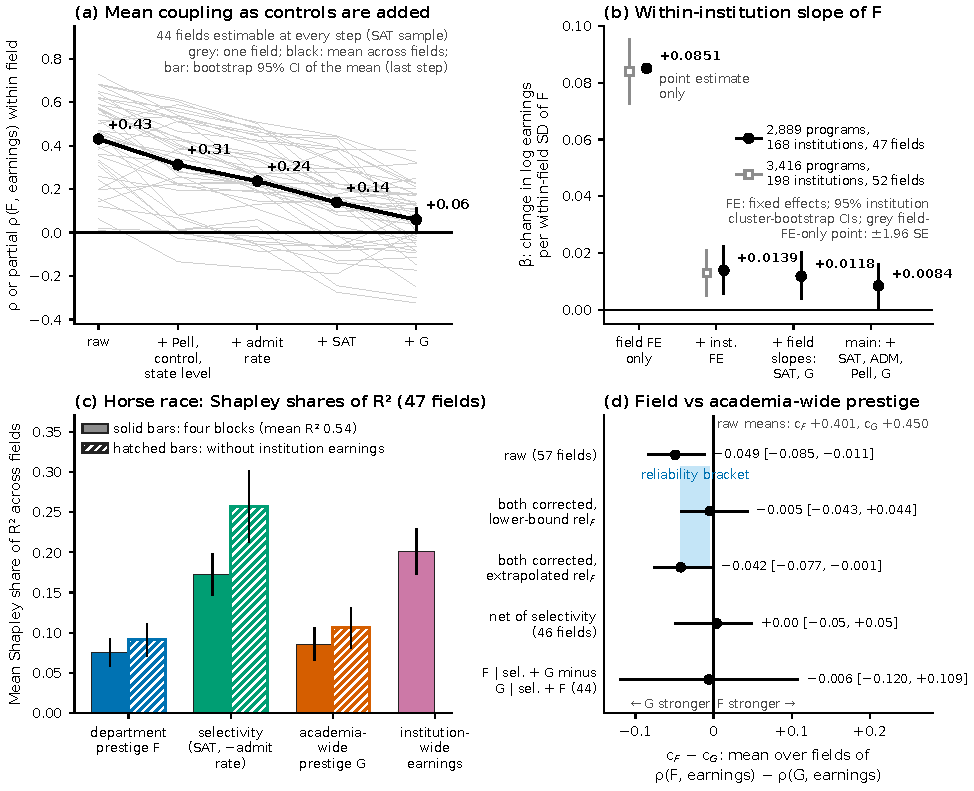
\includegraphics[width=0.64\linewidth]{../../outputs/figures/paper_fig2.pdf}
\caption{US coupling after university-level controls (Scorecard four-year pay; $F$ and $G$ are labelled
``department'' and ``academia-wide prestige''). (a) Mean coupling as controls are added (44 fields; grey: single
fields). (b) Within-institution slope of log pay per SD of $F$, from field fixed effects to the main specification.
(c) Mean Shapley shares of $R^2$, with and without (hatched) institution-wide earnings. (d) $c_F-c_G$: raw,
corrected for error in $F$, and net of selectivity. 95\% institution-bootstrap intervals.}\label{fig:status}
\end{figure}

The academic ranking is the published SpringRank hiring rank of \citet{wapman2022quantifying}, from a census of
faculty at 368 PhD-granting US institutions in 2011--2020 \citep{wapman2022data}. We use its field rank $F_{if}$ and
university-wide rank $G_i$, signed so that higher means higher standing. The pay ranking uses the median earnings $Y$
of each programme's bachelor's graduates. US sources are College Scorecard medians four years after completion (3,444
programmes in 52 fields; \citealp{scorecard}) and PSEO medians one, five and ten years after graduation for fixed
cohorts (39 fields; \citealp{pseo, pseo2026}). Scorecard medians cover only completers who received federal (Title
IV) aid and who work and are not enrolled. PSEO (unemployment-insurance wage records) and UK LEO (tax records) lack
the aid restriction; PSEO orders fields' coupling much as Scorecard does (Spearman $+0.68$, 57 fields), but the
within-institution slope rests on Scorecard alone. LEO medians are also released by graduates' prior-attainment band
(33 subjects, 134 providers; \citealp{dfe_leo_provider}). The UK has no field rank; its $G$ is a SpringRank of 11,987
PhD-to-faculty moves in ORCID-derived records \citep{li2026orcid}. Intake selectivity is mean SAT and admission rate
in the US, and the share of graduates with 360 or more UCAS points in the UK.

Partial coupling correlates the rank residuals of $F$ and $Y$ on the ranks of the controls. The reliability of $F$
lies between 0.81 and 0.96. Brackets are 95\% intervals that resample or cluster by institution (PSEO: two-way field
and institution clusters; UK: subjects, then providers).\footnote{The canonical sample is the 52 fields with at least
15 matched institutions; heterogeneity, reliability and $F$-against-$G$ statistics use the 57 with at least 8. Other
samples: the control ladder, 44 fields estimable at every step; the within-institution slope and Shapley shares, 47
with SAT data; the career analysis, 39 in the balanced PSEO panel; the field-map check, the 23 largest. UK: 33
subjects with at least 15 providers, 28 for same-band comparisons.} SI~S$n$ refers to the supplementary information
of the full-length paper. Two tests qualify what $F$ measures. T0 finds that $F$ partly reflects doctoral production:
residualised on production, $F$ keeps 0.598 \ci{0.471}{0.725} of its coupling, a lower bound because the
residualisation also removes net export that valuation itself produces. At most about two fifths of coupling thus
runs through production; the within-institution slope has not been re-estimated net of it. T1 finds that $F$ does not
order departments alike as placers and as hirers of PhDs, so we read it as a net-placement position, not one index of
doctoral quality.

% =====================================================================================
\section{Results}\label{sec:results}

\subsection{The two rankings agree, to a degree that varies by field}\label{sec:res-map}

Across the 52 US fields, mean coupling of $F$ with four-year pay is $+0.419$ \ci{+0.355}{+0.482} (SI~S3). It lies
more than 1.96 bootstrap standard errors above zero in 39 fields and below zero in none, from $+0.71$ in computer
science to $+0.07$ in nursing. The field map follows how closely each field's pay tracks mean SAT (true-score
correlation $+0.94$, 23 fields), as it would if fields differed only in the scale at which they price one
university-level index (Corollary~\ref{cor:thy-onefactor}; a consistency check, not a test). It therefore cannot
separate a department gradient in pay from a gradient in university status.

\subsection{Agreement sits at the university level and is largely shared with intake selectivity}\label{sec:res-name}

Mean SAT and admission rate alone lower mean US coupling from $+0.43$ to $+0.14$ (47 fields); Pell share, control and
state earnings level alone lower it to $+0.31$ (Fig.~\ref{fig:status}a). In per-field rank regressions, selectivity's
mean Shapley share of $R^2$ is 0.173, against 0.076 for $F$, 0.086 for $G$ and 0.201 for institution-wide earnings,
which contain the field's own graduates (Fig.~\ref{fig:status}c).

Before any control, $G$ couples with pay slightly more strongly than $F$ does: $c_F-c_G=-0.049$ \ci{-0.085}{-0.011}
(57 fields; Fig.~\ref{fig:status}d). At the across-field means, $\mathrm{sr}_F$ is 0.077 against a threshold of 0.156
(field by field they average 0.055 and 0.141), and $F$ out-predicts $G$ in only 15 of 57 fields
(Proposition~\ref{prop:thy-level}). Corrected for error in $F$, the difference is $-0.005$ \ci{-0.043}{+0.044} at the
lower-bound reliability; under either correction, and net of selectivity, $F$ does not detectably out-predict $G$,
though a small advantage is not excluded.

Within universities, the department's part of the agreement is small. With field fixed effects alone, one
within-field standard deviation (SD) of $F$ goes with $+0.084$ log points of four-year pay; institution fixed effects
lower this to $+0.013$ (Fig.~\ref{fig:status}b). The main specification adds field-specific slopes on mean SAT,
admission rate, Pell share and $G$; one SD of $F$ then goes with $+0.0084$ log points \ci{+0.0000}{+0.0164}, about
0.84\% (2,889 programmes; \ci{-0.0012}{+0.0180} under the two-way variance; about zero with one- and five-year
medians, which describe other cohorts). The upper 95\% limit is 1.6--1.8\% per SD of the observed rank. The controls
absorb most of $F$, and the part they leave has a reliability of about 0.3 at the lower bound; corrected for it, the
slope is about 3\% ($+0.0297$), so the department's part is diluted, not shown to be absent. Because US selectivity
is measured for the university, the slope also carries any sorting of stronger students into a university's
higher-ranked departments, of unknown sign; a control for the programme's own Pell share does not lower it, and
comparing majors that restrict entry with open majors is too weak to separate the two (SI~S4). Only computer science
has an individually clear remainder, $+0.050$ log points per SD \ci{+0.012}{+0.096}, pooled over horizons (128
programmes; the sample lacks 21 of the 50 highest-ranked departments, among them the University of California
campuses).

\subsection{In the UK, most agreement survives a control for graduates' prior attainment}\label{sec:res-uk}

The UK data add pay by graduates' own prior attainment, but no field rank, so they bear on the university level only.
Coupling of $G$ with five-year pay averages $+0.486$ \ci{+0.398}{+0.559} across 33 subjects. Among graduates of the
same attainment band coupling is $+0.227$, against $+0.342$ for all graduates of the same providers, so 66\%
\ci{51}{79} survives (28 subjects; 87\% \ci{74}{100} on 27 subjects after correcting for noise in band medians). The
band comparison controls graduates' own attainment, whereas institution-mean selectivity also removes peer and
resource effects: net of institution-level selectivity instead, UK coupling keeps 26\% ($+0.131$), a fall comparable
to the US one. If the UK $G$ is measured with little error, what remains within bands tracks intake selectivity at
least as closely as $G$. Selectivity keeps a same-band partial coupling of $+0.252$ \ci{+0.172}{+0.310} net of $G$,
while $G$ net of selectivity, itself a status measure, is $+0.033$, not distinguishable from zero (28 subjects). At a
validity of 0.74, however, the data allow $G$'s same-band partial to reach $+0.26$.

\subsection{Agreement rises with years since graduation and is weak under national pay scales}\label{sec:res-time}

Within fixed US graduation cohorts, coupling rises by $+0.031$ \ci{+0.021}{+0.041} per year since graduation (39
fields; PSEO), and UK coupling rises by about as much. The rise mixes career time with calendar time, and about three
fifths of the US rise is shared with entry-year selectivity. Graduate study is not excluded: if graduates of
higher-status universities more often leave the earnings data to study and return with higher pay, coupling rises
mechanically. With coverage and the university's research-doctorate rate as controls the slope falls from $+0.0305$
to $+0.0103$ per year, though that rate tracks $G$; coverage alone removes about a fifth, and a fifth to a third of
the rise moves with where graduates work (T7). Within the model, a rise at well-known universities needs earnings
growth, falling pay variance unrelated to $F$, or learning about departments, which is small since $\mathrm{sr}_F$ is
(Proposition~\ref{prop:thy-time}); outside it, graduate study, coverage and migration can produce the same rise.

Coupling is weak in UK subjects paid largely on national scales: nursing, medicine and teaching couple at $+0.120$,
against $+0.523$ for the other subjects (difference $-0.404$ \ci{-0.566}{-0.238}). Allied health, much of it also
paid on national bands, is an exception at $+0.570$, as is US special education ($+0.55$). A schedule that only
rescales market pay leaves correlations unchanged (Proposition~\ref{prop:thy-time}), so weak coupling reflects
noisier medians, schedule variance unrelated to status or weaker market agreement; these data do not separate them.

% =====================================================================================
\section{Discussion}\label{sec:discussion}

For a student choosing among university $\times$ field programmes, a department's academic reputation predicts little
of graduates' pay beyond the university's rank and intake: about 0.8\% per SD, with an upper 95\% limit of
1.6--1.8\%, or about 3\% once corrected for error in the rank. Computer science may be the exception. Subject
rankings built on academic standing may share this limit: $F$ plays that part here, and \citet{britton2022how} find a
similar pattern for UK league tables, none of whose subject ratings correlates positively and significantly with
returns net of intake.

Agreement is not a return: the university terms in (\ref{eq:thy-decomp}) can be pure common causes. At an
admission cutoff, the model splits the effect of admission to programme $p$ over a fallback $p'$ in the same field
into
\begin{equation}\label{eq:thy-cutoff}
\tau(t)=\Delta\delta+(1-\lambda_t)(\Delta R-\Delta\delta)+\beta_f\Delta g(t)
\end{equation}
(Corollary~\ref{cor:thy-cutoff}): value added, a reputation rent that employers pay even for a pure signal and that
learning erodes \citep{altonji2001employer, arcidiacono2010beyond, macleod2017big}, and growth. Cutoff data can
answer two questions. First, in data like those of \citet{anelli2020returns}, does the admission effect decline with years
since graduation, a rent that employers learn away, or rise through growth? The profile of $\tau(t)$ separates the two
(Corollary~\ref{cor:thy-cutoff}(iii)); rising cross-sectional coupling does not. Second, across many programme
cutoffs, does the effect differ with the fallback's department-rank gap, among fallbacks at universities of similar
standing?

One university's cutoff answers only the first: its rejected applicants go elsewhere, so it contrasts universities,
and the changed field choice through which part of Anelli's premium runs is a channel within that contrast. The
second needs ranked application lists, which identify each fallback \citep{kirkeboen2016field} and reveal students'
own ordering of programmes \citep{avery2013revealed}, and a department rank where cutoffs exist. $F$ exists only for
the US, which lacks programme cutoffs, but a hiring rank can be built from ORCID-derived moves, as our UK $G$ was.
Because $F$ and $G$ correlate 0.786 on average, the department-rank gap varies little given the university-rank gap,
so many cutoffs are needed. Projected on the target-minus-fallback gaps in the two reputations and in peer ability,
cutoff estimates of $\tau$ would show how much of a return goes with the university's standing and how much with the
department's; the model has no channel from academic standing to pay, so these loadings describe association across
cutoffs, not causal channels (Appendix~\ref{app:thy:design}). Earnings must span a decade or more: first-year medians
are distorted by graduate study and coverage, and the rent should erode while growth may rise. Which reputation
students themselves follow when they choose a programme is the next study's question.

\paragraph{Limitations.} The analysis uses public aggregates and does not separate value added, selection and
employer screening, nor say why agreement below the university is weak. It assumes, without testing, that pay equals
expected productivity. Programme medians miss the upper tail, where elite returns concentrate
\citep{zimmerman2019elite, chetty2023diversifying}, and PSEO lacks most of the top quartile of ranked institutions.
Pay is not netted of where graduates work: only raw five-year PSEO coupling was checked net of the wage level of
graduates' destination census divisions (unchanged, T7); the Scorecard ladder, partial couplings and
within-institution slope were not, and location within divisions is never netted. Selectivity is measured for the
university, not the programme, and whatever the proxies miss stays in every partial coupling. About a fifth of pay
coupling runs between employer sectors, which reflects employers' valuation only if employers ration access to
sectors. The UK hierarchy rests on self-reported ORCID careers of uncertain validity. The model's tests share data
with results already seen, and two of them are inconclusive for lack of power.

\bibliographystyle{plainnat}
\bibliography{../refs_merged,refs_short}

\clearpage
\appendix
% =====================================================================================
% theory_appendix.tex -- proofs for theory_core.tex (short draft of "Degrees of Separation"; author: Sora Yng).
% Written 2026-09-25; revised the same day after two referee reports (notes in comments at the end). Restates and
% tightens paper/si.tex Section S11; every number is copied from paper/si.tex, paper/main.tex, THEORY_NOTES.md or a
% repo-root *_RESULT.md; none is new. Labels: app:thy, tab:thy-rankings, prop:thy-*, lem:thy-*, rem:thy-*, cor:thy-*.
% Needs amsmath, array, booktabs and natbib. The environments and macro below are defined only if absent.
% =====================================================================================
\makeatletter
\@ifundefined{thylemma}{\newtheorem{thylemma}{Lemma}}{}
\@ifundefined{thyremark}{\newtheorem{thyremark}{Remark}}{}
\@ifundefined{thycor}{\newtheorem{thycor}{Corollary}}{}
\@ifundefined{thyaprop}{\newtheorem{thyaprop}{Proposition}}{}
\makeatother
\renewcommand{\thethylemma}{A\arabic{thylemma}}
\renewcommand{\thethyremark}{A\arabic{thyremark}}
\renewcommand{\thethycor}{A\arabic{thycor}}
\renewcommand{\thethyaprop}{A\arabic{thyaprop}}
\providecommand{\ci}[2]{$[#1,\allowbreak\,#2]$}
\providecommand{\thyqed}{\hfill$\square$}

\section{Proofs for Section~\ref{sec:thy}}\label{app:thy}

Moments are taken within field $f$ over $i\in\mathcal I_f$. $X^{\perp Z}$ is the residual of $X$ on $Z$, and
$\sigma_X^2=\mathrm{Var}\,X$. The university level is called the name. The tests T0--T8 were specified before the analysis; they are not publicly registered.

\begin{table}[!htbp]
\centering
\caption{Three revealed rankings of the same programmes. Audits: tests specified before the analysis; not publicly
registered.}\label{tab:thy-rankings}
\footnotesize
\begin{tabular}{@{}>{\raggedright\arraybackslash}p{2.1cm}>{\raggedright\arraybackslash}p{2.4cm}>{\raggedright\arraybackslash}p{3.4cm}>{\raggedright\arraybackslash}p{4.0cm}>{\raggedright\arraybackslash}p{2.7cm}@{}}
\toprule
Evaluator & Revealing choice & Indicator & Identifying assumption & Audit \\
\midrule
Hiring committees (academic market) & net direction of faculty hires & $F_{if}$ field rank, $G_i$ university-wide rank
\citep{wapman2022quantifying} & gravity model (H2); H0 volume neutrality reads $s^*$ as the valuation $s$ & T0 partly
production; T1 not one index \\
Employers (graduate market) & wages & $Y_{if}(t)$, programme median log earnings $t$ years after graduation & M1 pay
equals the posterior mean of productivity; M2 institution and major seen; M3 no pay schedule; M4 median covers
market workers & T7 location-robust; T8 between-sector share 0.21 \\
Students & applications and matriculation under capacity & $S_i$, mean SAT and admission rate (UK: share of
graduates with $\ge$360 UCAS points; LEO earnings by prior-attainment band within provider $\times$ subject) & S1
common ranking, admission by measured ability; defined for programmes only where admission is by programme (UK
UCAS, Norway, Chile, China) & none: the least audited leg \\
\bottomrule
\end{tabular}
\end{table}

\subsection{Assumptions}\label{app:thy:assumptions}

\begin{description}
\item[A0 (Gaussian copula).] The model holds for the normal scores of the latent components and the indicators, which
are jointly Gaussian. For two such variables with Pearson correlation $r$, Spearman's
$\rho=\tfrac{6}{\pi}\arcsin(r/2)$ \citep{kruskal1958ordinal}, which is strictly increasing. Statements about signs
and orderings therefore hold for $\rho$; magnitudes are statements about normal scores. Near zero, a rank-based
partial correlation need not have the sign of the latent one.
\item[E (classical errors).] $F=s^*+e_F$ (on the scale of $s^*$, Proposition~\ref{prop:thy-springrank}),
$G=a+e_G$, $Y(t)=m(t)+e_Y$ and $S=\xi+e_S$, with errors of mean zero, independent of one another and of every
latent variable; $\mathrm{rel}_X$ is the latent share of $\mathrm{Var}\,X$. The production component that T0 finds
is part of $s^*$, not of $e_F$. $S$ and $G$ aggregate an institution's programmes, so $e_S$ contains
$w_{if}y_{if}$ and $e_G$ a hire-weighted share of $r_{if}$, with $w_{if}$ the programme's share of its institution;
E holds up to terms of that order.
\item[A-orth (no covariance across levels).] $r_{if}$ and $y_{if}$ are uncorrelated with every university-wide
variable: $a_i$, $\xi_i$, $v_i$, $g_i(t)$ and employers' name belief $\hat x_i$, up to terms of order
$\max_gw_{ig}$ (Lemma~\ref{lem:thy-umbrella}). Defining $r$ and $y$ as within-field residuals delivers
$\mathrm{Cov}(a,r)=\mathrm{Cov}(x,y)=0$ and nothing more; the rest is assumed. It fails if departments are relatively
strong at selective institutions ($\mathrm{Cov}(r,\xi)>0$) or if high-status institutions draw relatively able
students into the major ($\mathrm{Cov}(a,y)>0$).
\item[H0--H2 (academic market).] $A_{uv}$ counts field-$f$ faculty at $v$ with a doctorate from $u$ ($u\neq v$).
Gravity: $\mathbb EA_{uv}=p_uh_v\,\varphi(s_u-s_v)\,\zeta_{uv}$, with origin and destination parameters
$p_u,h_v>0$, $\varphi$ positive, strictly increasing and differentiable, $\zeta_{uv}=\zeta_{vu}\ge0$ (geography,
subfield overlap), and no ties in $s$. Let $\pi_u=\log(p_u/h_u)$. The parameters $p,h$ are not the observed volumes:
the expected number of $u$'s doctorates placed, $p_u\sum_vh_v\varphi(s_u-s_v)\zeta_{uv}$, also depends on $s$. H0
(volume neutrality): $\pi_u$ is the same for all departments. H1 (vertical sorting): for every pair with
$\zeta_{uv}>0$, $s_u>s_v$ implies $\mathbb EA_{uv}>\mathbb EA_{vu}$. H2 (many hires): $\mathbb EA_{uv}=n\alpha_{uv}$
with $\alpha$ fixed and $A_{uv}/n\to_p\alpha_{uv}$ as $n\to\infty$. Under the gravity form H0 implies H1, since
$\mathbb EA_{uv}/\mathbb EA_{vu}=\exp(\pi_u-\pi_v)\,\varphi(\Delta)/\varphi(-\Delta)$ with $\Delta=s_u-s_v$, and
$\varphi(\Delta)>\varphi(-\Delta)$ for $\Delta>0$.
\item[M1--M4 (graduate market).] Graduate $k$ of programme $p=(i,f)$ has productivity $\eta_k=\theta_p+\varepsilon_k$,
$\varepsilon_k\sim N(0,\sigma^2)$ independent, plus growth $\beta_fg_i(t)$. M1: employers compete, and pay is the
posterior mean of productivity given their information \citep{farber1996learning}: the credential, the graduate's
own signals (precision $h_b$ at hiring, $h_\varepsilon$ in each later year), a public signal $P_i$ about the name,
and records of past graduates' performance attributed to units. Attribution is costly or markets are segmented, so a
unit's record counts the graduates a local market has attributed to it. M1 includes four conditions. (i) Learning
is symmetric: employers competing in a local market share the same records and signals; with employer-specific
information the competitive wage need not be the posterior mean
\citep{waldman1984job,greenwald1986adverse,schonberg2007testing,kahn2013asymmetric}. (ii) The prior precision $h_0$
of $\eta_k$ given the programme's record is the same across programmes. This is an approximation for when $\sigma^2$
dominates the prior variance of $\theta$ given the record, $\beta_f^2(1-\omega_i)\tau_i^2+(1-\omega_f)\tau_y^2$,
which varies with the weights of Lemma~\ref{lem:thy-umbrella}. (iii) Growth is known to employers and $g_i(0)=0$.
(iv) $\omega_{if}$ is constant within a field, or independent of $r$ and $y$ (programme size, which sets the
attributed record, may vary with status). M2: the institution and the major are seen at hiring. M3: pay is not set
by a schedule. M4: the programme median equals mean log pay among graduates in the employer market, and programmes
are large enough that averages of $\varepsilon_k$ and of signal noise vanish.
\item[S1 (students).] Programmes $j=1,\dots,J$ with capacities $q_j$; applicants with distinct measured abilities
$\tilde a_k$. All applicants rank programmes in the same strict order $1\succ2\succ\dots\succ J$ and prefer any
programme to none; every programme admits by measured ability up to capacity.
\end{description}

\subsection{The academic market}\label{app:thy:academy}

\begin{thyaprop}[SpringRank's large-sample limit]\label{prop:thy-springrank}
Assume the gravity form, H2, and that the exchange graph (pairs with $\alpha_{uv}+\alpha_{vu}>0$) is connected. Let
$\hat s_n$ be the SpringRank scores of $A$ as the ridge vanishes, centred. Then $\hat s_n\to_p\hat s$, the centred
solution of
\[
\sum_vK_{uv}(\hat s_u-\hat s_v)=\sum_vK_{uv}\tanh z_{uv},\qquad
z_{uv}=\tfrac12(\pi_u-\pi_v)+\tfrac12\{\log\varphi(s_u-s_v)-\log\varphi(s_v-s_u)\},
\]
with $K_{uv}=\alpha_{uv}+\alpha_{vu}$. To first order in $z$, $\hat s=c_\varphi s+\tfrac12\pi+\text{const}$ with
$c_\varphi=(\log\varphi)'(0)$, so $\hat s/c_\varphi=s^*:=s+\pi/(2c_\varphi)$ up to a constant. Under SpringRank's own
kernel, $\varphi(\Delta)\propto\exp\{-\tfrac{\beta}{2}(\Delta-1)^2\}$, $c_\varphi=\beta$ and
$z_{uv}=\beta(s^*_u-s^*_v)$ exactly, so the only approximation is $\tanh z\approx z$; where $|z|$ is large (a steep
hierarchy or very unequal volumes) $\tanh$ saturates and $\hat s$ can misorder some pairs relative to $s^*$. An
exchange between $u$ and $v$ goes from $u$ to $v$ with probability $\{1+\exp(-2z_{uv})\}^{-1}$, so directions
depend on $s$ and $\pi$ only through $z$ and cannot separate them; under SpringRank's kernel they identify $s^*$
exactly.
\end{thyaprop}

\emph{Proof.} SpringRank minimises $\tfrac12\sum_{uv}A_{uv}(\hat s_u-\hat s_v-1)^2$ plus a ridge
\citep{debacco2018physical}. Its first-order condition as the ridge vanishes is
$\sum_v(A_{uv}+A_{vu})(\hat s_u-\hat s_v)=\sum_v(A_{uv}-A_{vu})$, a Laplacian system whose centred solution is
unique and continuous in $A/n$ on connected graphs. By H2 and the continuous mapping theorem, $\hat s_n$ converges in
probability to the solution with $A/n$ replaced by $\alpha$. Under the gravity form $\zeta$ cancels from
$\alpha_{uv}/\alpha_{vu}=\exp(2z_{uv})$, so $(\alpha_{uv}-\alpha_{vu})/(\alpha_{uv}+\alpha_{vu})=\tanh z_{uv}$, which
gives the display. The odd part of $\log\varphi$ is $c_\varphi\Delta+O(\Delta^3)$ and $\tanh z=z+O(z^3)$, so to first
order the right side is $\sum_vK_{uv}\{c_\varphi(s_u-s_v)+\tfrac12(\pi_u-\pi_v)\}$, which $c_\varphi s+\tfrac12\pi$
solves; connectedness makes the solution unique up to a constant. Under SpringRank's kernel
$\log\varphi(\Delta)-\log\varphi(-\Delta)=2\beta\Delta$ exactly. The direction probability is
$\alpha_{uv}/(\alpha_{uv}+\alpha_{vu})$. \thyqed

Academic reputation is therefore defined as the revealed position $s^*$, an estimable parameter of the flow model,
so the definition is not circular. Reading it as the academy's valuation $s$ of the department is what H0 adds: H0
is an identifying normalisation, which only outside data on production and hiring can audit (T0), and those data
are proxies for $p$ and $h$, not the parameters themselves. We do not model the committees' expectation of doctoral
quality.

\begin{thylemma}[Minimum-violation ordering]\label{lem:thy-mvr}
For an ordering $\varpi$, let $V(\varpi)=\sum_{(u,v):\,v\succ_\varpi u}\mathbb EA_{uv}$ be the expected number of hires
that move up $\varpi$, and $V_n(\varpi)$ the sample count. Under H1, every minimiser of $V$ agrees with $s$ on every
exchanging pair and on every pair linked by a chain of exchanging pairs that is monotone in $s$. Under H1 and H2,
every minimiser of $V_n$ agrees with $s$ on those pairs with probability tending to one.
\end{thylemma}

\emph{Proof.} $V$ is a sum over unordered pairs. For a pair with $s_u>s_v$, an ordering that puts $v$ above $u$ adds
$\mathbb EA_{uv}$ to $V$, and the $s$-ordering $\varpi_s$ adds $\mathbb EA_{vu}$. Hence
$V(\varpi)-V(\varpi_s)=\sum_{\text{pairs inverted by }\varpi}(\mathbb EA_{uv}-\mathbb EA_{vu})\ge0$, with equality only
if $\varpi$ inverts no exchanging pair (H1). A minimiser is a total order, so it also agrees with $s$ along any
monotone chain of exchanging pairs; pairs linked by no such chain are left unordered by the data. There are finitely
many orderings; by H2, $V_n(\varpi)/n-V(\varpi)/n\to_p0$ for each, and $\{V(\varpi)-V(\varpi_s)\}/n$ is bounded away
from zero for every $\varpi$ that inverts an exchanging pair, so every sample minimiser
\citep{clauset2015systematic} agrees with $s$ on those pairs with probability tending to one. \thyqed

The lemma is close to a restatement of H1 and concerns the minimum-violation ordering, not the published $F$; what
links $F$ to $s$ is Proposition~\ref{prop:thy-springrank} together with H0.

\begin{thyremark}[H1, SpringRank and the minimum-violation ordering]\label{rem:thy-springrank}
(i) If $\varphi$ is constant (random matching, no valuation), $\mathbb EA_{uv}>\mathbb EA_{vu}$ if and only if
$\pi_u>\pi_v$: H1 holds for the ordering by production relative to hiring. H1 alone therefore does not reveal a
valuation; H0 does. (ii) The first-order condition in the proof of Proposition~\ref{prop:thy-springrank} reads
$\hat s_u=\bar s_u+(d^{\rm out}_u-d^{\rm in}_u)/(d^{\rm out}_u+d^{\rm in}_u)$, with $\bar s_u$ the exchange-weighted
mean of $u$'s partners: a department sits above its partners by its net-export ratio. (iii) Under H1, $F$ can
disagree with the minimum-violation ordering. Take $A_{uv}=1$, $A_{vu}=0$, $A_{vw}=100$, $A_{wv}=0$, $A_{uw}=100$
and $A_{wu}=99$. H1 holds for $u\succ v\succ w$, and the minimum-violation ordering is $u\succ v\succ w$ (99 upward
hires; every other ordering has at least 100). SpringRank gives $s_v-s_w=0.98$ and $s_u-s_w=0.015$, so
$v\succ u\succ w$. On the public edges, $F$ correlates $+0.662$ on average with a minimum-violation ordering.
\end{thyremark}

\begin{thyremark}[Audits of H0 and H1]\label{rem:thy-audits}
T0 replaces $F$ by a degree-corrected Bradley--Terry rank (offsets
$\log\{d^{\rm out}_ud^{\rm in}_v/(d^{\rm out}_vd^{\rm in}_u)\}$) and by $F$ residualised on log doctoral production and
the export ratio. Coupling keeps $R_{\mathrm{DC}}=0.839$ \ci{0.743}{0.936} and $R_\perp=0.598$ \ci{0.471}{0.725} of
its size: ``partly production''. $1-R_\perp$ bounds the share of coupling carried by the production term of
Proposition~\ref{prop:thy-agree} from above, because residualising also removes the net export that valuation
itself produces (H1), but only if $F$'s production component lies (linearly) in the span of the two regressors. By
Proposition~\ref{prop:thy-springrank} that component is $\tfrac12\log(p/h)$, which the regressors span only
approximately, and observed volumes only proxy $p$ and $h$; the audit is to be read with $\log(p/h)$. T1 asks whether one index orders departments both by where their
doctorates are placed and by where their faculty come from: $R=0.525$ \ci{0.461}{0.583} against a threshold of 0.80,
and $R'-R_0=-0.169$ \ci{-0.229}{-0.115} against a benchmark from SpringRank's own generative model (``not one
index''; the benchmark's calibration was fixed after the literal one had degenerated). The faculty market is
two-sided: flows reflect committees' valuation of degree-granting departments and candidates' preferences over
employers. If committees rank candidates by $s_u$ and candidates rank employers by an index $t_v$, flows depend on
$s_u$ and $t_v$, and ``not one index'' reads as $t\neq s$; we do not build that model. A network position or placement
power predicts the same agreement of roles, so T1 cannot separate valuation from position; only T0 speaks to
production.
\end{thyremark}

\subsection{The graduate market}\label{app:thy:market}

\begin{thylemma}[Attribution weights]\label{lem:thy-umbrella}
Let the employers of a local market share a record of $n^e_{ig}$ graduates of each programme $(i,g)$, with
$n^e_i=\sum_gn^e_{ig}$ and $w_{ig}=n^e_{ig}/n^e_i$. Measured in field-standardised units, $(\eta_k-\mu_g)/\beta_g$, the
name's pooled record has mean $x_i+\bar u_i+\nu_i$, with $\bar u_i=\sum_gw_{ig}y_{ig}/\beta_g$ and noise $\nu_i$ of
variance $\bar\sigma^2/n^e_i$, $\bar\sigma^2=\sum_gw_{ig}\sigma^2/\beta_g^2$. Give $x_i$ a normal prior with mean
$p_i=\mathbb E[x_i\mid P_i]$ and variance $\tau_i^2$, and let department deviations, with prior variance $\tau_y^2$,
be learned as deviations from the name's mean from the $n^e_{if}\delta_f$ graduates attributed to $(i,f)$ ($\delta_f$
the attribution probability). Dropping terms in $\bar u_i$, which are common to the institution's programmes and
correlate with $y_{if}$ only through its weight $w_{if}$,
\[
\hat x_i=\omega_i(x_i+\nu_i)+(1-\omega_i)p_i,\qquad
\omega_i=\frac{n^e_i\tau_i^2}{n^e_i\tau_i^2+\bar\sigma^2},\qquad
\omega_f=\frac{n^e_{if}\delta_f\tau_y^2}{n^e_{if}\delta_f\tau_y^2+\sigma^2},
\]
and the belief about $y_{if}$ is $\omega_f(y_{if}+\nu_{if})$, with $\nu_{if}$ the department record's noise. Hence
$\omega_i\ge\omega_f$ whenever $\tau_i^2/\bar\sigma^2\ge\tau_y^2/\sigma^2$ (with $\beta_g\equiv1$, whenever
$\tau_i^2\ge\tau_y^2$), $\omega_i\to1$ as $n^e_i\to\infty$, and $\omega_f\to0$ as $\delta_f\to0$.
\end{thylemma}

\emph{Proof.} A record of $n$ observations of a unit has mean equal to the unit's value plus noise of variance
(per-observation variance)$/n$, and normal updating from a prior of variance $\tau^2$ gives the posterior mean
$\omega\cdot\text{record}+(1-\omega)\cdot\text{prior mean}$ with $\omega=n\tau^2/(n\tau^2+\text{per-observation
variance})$. The name's record pools all $n^e_i$ graduates; a department's record holds the $n^e_{if}\delta_f$
attributed to it. The map $n\tau^2\mapsto n\tau^2/(n\tau^2+c)$ is increasing, and $n^e_i\ge n^e_{if}\delta_f$.
\thyqed

Institution fixed effects absorb $\bar u_i$, and A-orth and the results below hold up to terms of order
$\max_gw_{ig}$. The record noise is kept: $\hat x$ is then a posterior mean and uncorrelated with its own error
$x-\hat x=(1-\omega_i)(x-p)-\omega_i\nu_i$. The noise terms are independent of $F$, $G$, $S$ and every latent
variable, so they enter no covariance used in Propositions~\ref{prop:thy-agree}, \ref{prop:thy-level} and
\ref{prop:thy-time}, Corollaries~\ref{cor:thy-onefactor}--\ref{cor:thy-decay} or the ratio of
Remark~\ref{rem:thy-y1}; they enter $\mathrm{Var}\,m(t)$, and hence any coefficient standardised by it.

\begin{thylemma}[Programme wage]\label{lem:thy-wage}
Under M1--M4, with $R_{if}=\beta_f\hat x_i+\omega_f(y_{if}+\nu_{if})$ (Lemma~\ref{lem:thy-umbrella}),
\[
m_{if}(t)=\mu_f(t)+V_{if}(t)+\beta_fg_i(t),\qquad V_{if}(t)=(1-\lambda_t)R_{if}+\lambda_t\theta_{if},\qquad
\lambda_t=b+(1-b)\frac{t}{t+k},
\]
with $b=h_b/(h_0+h_b)$ and $k=(h_0+h_b)/h_\varepsilon$. Equivalently
$m_{if}(t)-\mu_f(t)=\beta_fM_i(t)+\Lambda_{ft}\,y_{if}+(1-\lambda_t)\omega_f\nu_{if}$, with
$M_i(t)=(1-\lambda_t)\hat x_i+\lambda_tx_i+g_i(t)$ and $\Lambda_{ft}=\omega_f+(1-\omega_f)\lambda_t$; the
university-wide part of pay is $m^U_{if}(t)=\beta_fM_i(t)$.
\end{thylemma}

\emph{Proof.} After the hiring signal and $t$ yearly signals, normal updating gives the posterior mean
$(1-\lambda_t)R_{if}+\lambda_t\bar z_k$, where $\bar z_k$ is the precision-weighted mean of $k$'s signals, which is
$\eta_k$ plus noise, and $\lambda_t=(h_b+th_\varepsilon)/(h_0+h_b+th_\varepsilon)$; direct algebra gives
$\lambda_t=b+(1-b)t/(t+k)$. By M1(iii) the wage adds the known growth. Averaging over the programme's graduates
removes $\varepsilon_k$ and the signal noise (M4), and M4 equates the median with the mean; the average posterior
mean is $V_{if}(t)$. Substituting $\theta_{if}=\beta_fx_i+y_{if}$ and $R_{if}$ and collecting the coefficient of
$y_{if}$, $(1-\lambda_t)\omega_f+\lambda_t=\Lambda_{ft}$, gives the second form. \thyqed

\emph{Employer reputation.} $V_{if}(t)$, the graduate market's mean belief about the productivity of the programme's
graduates at $t$, equals $m_{if}(t)-\mu_f(t)-\beta_fg_i(t)$ under M1--M4, so it is revealed at every $t$ once growth
is known. \emph{Entry reputation} is $R_{if}=V_{if}(0)$; since $g_i(0)=0$, at entry with $b=0$ pay reveals it. The
\emph{reputation premium} $R-\theta$, the object of \citet{macleod2017big}, decays with learning,
$V(t)-\theta=(1-\lambda_t)(R-\theta)$. At a name with $\omega_i=1$, $V-\theta=-(1-\lambda_t)(1-\omega_f)y_{if}$ up to
record noise, so the university-wide parts of $V$ and $\theta$ coincide and pay at the name ranks selection-inclusive
expected productivity. In the data, employer reputation is programme earnings as priced by the graduate market,
selection included; it differs from mean productivity only where $\omega<1$ or at entry, and these data measure
neither: M4 fails most at one year (Remark~\ref{rem:thy-y1}). Under M1 with a public and costless record, every
graduate ever observed would enter the record, and $\omega_f$ would be close to one unless $\tau_y^2$ were tiny, which
is itself a statement of little departmental content; a small $\omega_f$ needs costly attribution or segmented
records.

\emph{College reputation in economics.} \citet{macleod2017big} measure a college's reputation by the mean admission
score of its graduates, find that it is correlated with graduates' earnings growth, and find that a new public signal
of individual skill, a college exit exam, lowered its return. The within-band rise found here (T4: the partial
correlation of pay with selectivity given $G$ rises by $+0.0266$ \ci{+0.0157}{+0.0374} per year within fixed cohorts,
on average over bands, concentrated in the middle bands) is in line with the first finding. \emph{Growth.} If growth
is complementary with ability, $g_i(t)=\gamma_tx_i$ with $\gamma_0=0$, it loads on the same $x$ that sets the level,
selectivity included, which is in line with T4; this is one specification of the growth slot, not a test of it, and
M1(iii) then requires $x_i$ to be known, as it is where $\omega_i=1$.

\subsection{Students}\label{app:thy:students}

\emph{Choice.} Student $k$, with ability $a_k$ and measured ability $\tilde a_k$, values programme $p$ at
$u_k(p)=\mathbb E_k[w_p(a_k)\mid\Sigma_k]+\varepsilon_{kp}$, where $\Sigma_k$ are the signals $k$ sees (rankings of
the academic-reputation kind, published programme earnings, intake statistics) and $\varepsilon_{kp}$ is taste.
Write $U_p$ for the part common to all students, the programme's reputation among students. Programme $p$ admits
applicants with $\tilde a_k\ge c_p$, and cutoffs clear capacity, so $c_p$ and intake ability $\xi_p$ are
equilibrium outcomes. S1 is the case $\varepsilon\equiv0$: then students rank programmes by $U_p$, and by
Lemma~\ref{lem:thy-students} $\xi_p$ is an increasing function of the rank of $U_p$. With tastes, comparative
advantage or strategic application the ordering holds only on average, and self-selection on gains
\citep{kirkeboen2016field} breaks it. Which of academic reputation, employer reputation, peer ability and value added
$U_p$ loads on is the next study's question; for schools, \citet{abdulkadiroglu2020parents} ask whether parents'
choices follow school effectiveness or peer quality.

\begin{thylemma}[Selectivity as a revealed ranking]\label{lem:thy-students}
Under S1 the stable matching is unique \citep{gale1962college}. It assigns the $q_1$ applicants of highest measured
ability to programme 1, the next $q_2$ to programme 2, and so on. Every entrant of programme $j$ then has higher
measured ability than every entrant of programme $j+1$, so the mean, the median and every other location statistic of
measured intake ability order programmes as students' common ranking does. If the distribution of $a$ given
$\tilde a$ is increasing in $\tilde a$ in the sense of first-order stochastic dominance (implied by the monotone
likelihood ratio property, and by jointly Gaussian $a$ and $\tilde a$ with positive correlation), and admission
depends on $a$ only through $\tilde a$, the mean and every quantile of true intake ability order programmes in the
same way.
\end{thylemma}

\emph{Proof.} Existence: in the serial assignment $\mu^*$, an applicant $k$ who prefers $j$ to $\mu^*(k)$ has $j$
ranked above $\mu^*(k)$; $j$ was filled before $k$ was placed, and only with applicants of higher ability than $k$, so
$j$ does not want $k$, and $\mu^*$ has no blocking pair. Uniqueness, by induction on $J$: let $\mu$ be stable and let
$k$ be among the $q_1$ highest-ability applicants. If $\mu(k)\neq1$, then $k$ prefers programme 1, and programme 1
either has a free seat or holds an applicant of lower ability than $k$; either way $(k,1)$ blocks $\mu$. So programme 1
holds exactly the $q_1$ highest-ability applicants. Removing them and programme 1 leaves a stable matching of the
smaller market, to which the argument applies again. The ordering claim follows because the entrants of $j$ are all
placed before those of $j+1$. For true ability, the distribution of $a$ among entrants of $j$ averages
$\Pr(a\le z\mid\tilde a)$ over measured abilities that all exceed those of $j+1$; each such term is no larger, so the
distribution for $j$ dominates that for $j+1$ at every $z$. \thyqed

S1 is a sufficient condition, and it is strong. Admission and yield rates can be manipulated, which is why
\citet{avery2013revealed} rank colleges from the matriculation choices of students admitted to several. A
university $\times$ field ordering by students exists only where admission is by programme (UK UCAS by course,
Norway, Chile, China's national examination with cutoffs by institution and major). US students are admitted to an
institution and choose a major later, sometimes under major-specific grade restrictions \citep{bleemer2022will}, so the
US indicators (mean SAT, admission rate) are university-level: a capacity-weighted average over the institution's
programmes, with any field-specific part of students' ranking in $y_{if}$. UK LEO earnings by provider $\times$
subject $\times$ prior-attainment band carry a programme-level measure of intake.

\subsection{Proof of Proposition~\ref{prop:thy-agree}}\label{app:thy:p1}

\emph{Reliability.} By E, $\mathrm{Cov}(F,Y)=\mathrm{Cov}(s^*,m)$, $\mathrm{Var}\,F=\mathrm{Var}\,s^*/\mathrm{rel}_F$
and $\mathrm{Var}\,Y=\mathrm{Var}\,m/\mathrm{rel}_Y$, so on normal scores
$\mathrm{Corr}(F,Y)=\sqrt{\mathrm{rel}_F\mathrm{rel}_Y}\,\mathrm{Corr}(s^*,m)$; by A0, $\rho_f$ is a strictly
increasing function of it.

\emph{Decomposition.} By Lemma~\ref{lem:thy-wage}, $m-\mu_f=m^U+\Lambda_{ft}y$ plus record noise. Write
$s^*=\alpha_fa+r+\pi/(2\beta)$ and project on $\xi$:
$s^*=\{\mathrm{Cov}(s^*,\xi)/\sigma_\xi^2\}\,\xi+s^{*\perp\xi}$ with
$s^{*\perp\xi}=\alpha_fa^{\perp\xi}+r+\pi^{\perp\xi}/(2\beta)$, since $\mathrm{Cov}(r,\xi)=0$ (A-orth). By A-orth,
$\mathrm{Cov}(a,y)=\mathrm{Cov}(\xi,y)=0$, so $\mathrm{Cov}(a^{\perp\xi},m)=\mathrm{Cov}(a^{\perp\xi},m^U)$ and
$\mathrm{Cov}(\xi,m)=\mathrm{Cov}(\xi,m^U)$; and $\mathrm{Cov}(r,m^U)=0$, so
$\mathrm{Cov}(r,m)=\Lambda_{ft}\mathrm{Cov}(r,y)=\Lambda_{ft}\kappa_f\sigma_r\sigma_y$. Summing gives
(\ref{eq:thy-decomp}).

\emph{Partialling selectivity.} The partial covariance of $F$ and $Y$ given $S$ is
\[
\mathrm{Cov}(F,Y)-\mathrm{Cov}(F,S)\,\mathrm{Cov}(S,Y)/\mathrm{Var}\,S.
\]
By E, $\mathrm{Cov}(F,S)=\mathrm{Cov}(s^*,\xi)$,
$\mathrm{Cov}(S,Y)=\mathrm{Cov}(\xi,m)$ and $\mathrm{Var}\,S=\sigma_\xi^2/\mathrm{rel}_S$, so the subtracted quantity
is $\mathrm{rel}_S$ times the first term of (\ref{eq:thy-decomp}). The partial therefore exceeds the last three
terms, that is, bounds agreement beyond measured intake from above, if and only if $\mathrm{Cov}(s^*,\xi)$ and
$\mathrm{Cov}(\xi,m)$ have the same sign. \thyqed

Four remarks on use. (i) $\mathrm{Cov}(s^*,m)>0$ is not implied: it needs the two valuations to load in the same
direction on the university-wide components, and $\kappa_f$ and the production term not so negative as to offset.
(ii) The reported figures ($+0.43$ to $+0.14$) are mean partial correlations. A partial correlation divides the
partial covariance by residual standard deviations below the raw ones, so the share of covariance that runs through
$\xi$ is larger than the proportional fall in correlation. (iii) $e_S$ contains $w_{if}y_{if}$, so the partial is
exact only up to terms of that order (E). (iv) The first term is not selection alone: peer quality and resources
that rise with intake load on $\xi$, which is why \citet{dale2002estimating} treat selectivity as a candidate
treatment; programme aggregates cannot separate a graduate's own ability from her peers', because at the programme
mean they coincide. If students sort on reputation \citep{macleod2015reputation}, intake is partly an outcome of
$s^*$ and $R$, and partialling it removes the part of agreement that runs through attracting students. The UK
attainment-band comparisons control graduates' own prior attainment, in the sense of \citet{macleod2017big}; the US
partial on institution-mean SAT removes peer and resource effects as well, so the two are different objects.

\begin{thycor}[Fields as scales of one index]\label{cor:thy-onefactor}
Suppose that (a) $\lambda_t$ is common across fields, so that $m^U_{if}(t)=\beta_fM_i(t)$ with $M_i(t)$ the
same in every field (Lemma~\ref{lem:thy-wage}); (b) $\alpha_f$, $\sigma_r$ and the joint moments of $(a,\xi,M)$ over $\mathcal I_f$
are common to all fields; (c) $\kappa_f\approx0$ in covariance, while the field-specific variance
$\Lambda_{ft}^2\sigma_{y,f}^2$, the record noise and $e_Y$ may differ across fields; and (d) H0. Then the true-score
coupling of field $f$ and the true-score correlation of its pay with $\xi$ are both proportional to
\[
\frac{\beta_f}{\mathrm{sd}\,m_f}=\Bigl\{\mathrm{Var}\,M+\frac{\Lambda_{ft}^2\sigma_{y,f}^2+\text{noise variance}}{\beta_f^2}\Bigr\}^{-1/2},
\]
with a ratio, $\alpha_f\mathrm{Cov}(a,M)\,\sigma_\xi/\{\mathrm{Cov}(\xi,M)\,\mathrm{sd}\,s\}$, that is the same in
every field. The two field maps are therefore collinear, and both order fields by the share of programme pay variance
that is university-wide, not by the steepness of pricing; the same holds with any status index of this form in place
of $F$.
\end{thycor}

\emph{Proof.} By (c), $\mathrm{Cov}(s,m)=\alpha_f\beta_f\mathrm{Cov}(a,M)$, and
$\mathrm{Cov}(\xi,m)=\beta_f\mathrm{Cov}(\xi,M)$ by A-orth. Dividing by $\mathrm{sd}\,s\cdot\mathrm{sd}\,m_f$ and
$\sigma_\xi\,\mathrm{sd}\,m_f$ gives two correlations proportional to $\beta_f/\mathrm{sd}\,m_f$, and
$\mathrm{sd}^2m_f=\beta_f^2\mathrm{Var}\,M+\Lambda_{ft}^2\sigma_{y,f}^2+\text{noise variance}$. By (b), the ratio and
$\mathrm{sd}\,s=(\alpha_f^2+\sigma_r^2)^{1/2}$ do not depend on $f$. \thyqed

The assumption that fields differ only in the scale at which they price a common university-level index comes close
to the conclusion. The observed true-score correlation of the two maps, $+0.94$, is a consistency check, not a
prediction; replacing $F$ by three non-academic indices (T5) is inconclusive.

\subsection{Proof of Proposition~\ref{prop:thy-level}}\label{app:thy:p2}

\emph{Definitions and identity.} Standardise the ranks of $F$, $G$ and $Y$. Regress $F$'s standardised ranks on
$G$'s: the slope is $\cos\vartheta=\rho(F,G)$ and the residual is $\sin\vartheta\,H$, with $H$ of unit variance and
orthogonal to $G$. $\mathrm{sr}_F$ is the Pearson correlation of $Y$'s standardised ranks with $H$, not a Spearman
correlation of the residual, whose re-ranking would break the identity. By linearity,
$c_F=c_G\cos\vartheta+\mathrm{sr}_F\sin\vartheta$, and in the regression of $Y$ on $F$ and $G$ the coefficient on $F$
is $\mathrm{sr}_F/\sin\vartheta$ (Frisch--Waugh). Then $c_F-c_G=\mathrm{sr}_F\sin\vartheta-c_G(1-\cos\vartheta)$, which
is positive if and only if $\mathrm{sr}_F>c_G(1-\cos\vartheta)/\sin\vartheta=c_G\tan(\vartheta/2)$ for
$\vartheta\in(0,\pi)$. The identity holds for any three variables; the model enters only in reading $\mathrm{sr}_F$
and $c_G$.

\emph{Model reading.} ``$G=a$ up to negligible error'' requires, besides $\mathrm{rel}_G\approx1$, that the
published $G$, which pools the hires of all fields including $f$, carry a negligible hire-weighted mean of
field-specific deviations. That holds if field deviations are independent within an institution; if they are
correlated (a school layer, as in the SI), $G=a+\bar r^S$ with $\bar r^S$ not negligible and $F^{\perp G}\neq r+e_F$.
On normal scores with $G=a$ ($\mathrm{Var}\,a=1$) and H0, $F=\alpha_fa+r+e_F$, so $\cos\vartheta=\alpha_f/\mathrm{sd}\,F$
and $F^{\perp G}=r+e_F$, whose variance is $\sin^2\vartheta\,\mathrm{Var}\,F$. All of $F$'s error lies in
$F^{\perp G}$, since $e_F$ is independent of $G$; hence the reliability of $F^{\perp G}$ is
$\mathrm{rel}_H=\sigma_r^2/(\sigma_r^2+\sigma_{e_F}^2)=1-(1-\mathrm{rel}_F)/\sin^2\vartheta$, below $\mathrm{rel}_F$
whenever $\cos\vartheta\neq0$ and $\mathrm{rel}_F<1$. By Lemma~\ref{lem:thy-wage} and A-orth,
$\mathrm{Cov}(Y,F^{\perp G})=\mathrm{Cov}(m,r)=\Lambda_{ft}\kappa_f\sigma_r\sigma_y$, so
$\mathrm{sr}_F=\sqrt{\mathrm{rel}_H}\,\Lambda_{ft}\kappa_f\sigma_y/\mathrm{sd}\,Y$, and
$c_G=\mathrm{Cov}(a,m^U)/\mathrm{sd}\,Y$ because $\mathrm{Cov}(a,y)=0$. Agreement concentrates at the university
level ($c_G\ge c_F$) if and only if
$\sqrt{\mathrm{rel}_H}\,\Lambda_{ft}\kappa_f\sigma_y\le\tan(\vartheta/2)\,\mathrm{Cov}(a,m^U)$. Without H0,
$F^{\perp G}$ also carries $\pi^{\perp a}/(2\beta)$. \thyqed

At the across-field means ($\cos\vartheta=0.786$, $c_G=0.450$) the threshold is $0.156$ against
$\mathrm{sr}_F=0.077$, exceeded in 15 of 57 fields; on true scores the thresholds are 0.13 and 0.17 (lower-bound and
extrapolated reliability of $F$) against about 0.12 and 0.09. The within-institution slope,
$+0.0084$ \ci{+0.0000}{+0.0164} log points per SD of $F$ (\ci{-0.0012}{+0.0180} under the two-way
variance; about zero with one- and five-year medians), is individually clear only in computer science.

\emph{Entry and attribution.} By Lemma~\ref{lem:thy-wage}, at $t=0$ with $b=0$ the field-specific term is
$\omega_f\kappa_f\sigma_r\sigma_y$, non-zero if and only if $\kappa_f\neq0$ and $\omega_f>0$. For $t>0$ or $b>0$,
$\Lambda_{ft}\ge\lambda_t>0$, and the term is non-zero if and only if $\kappa_f\neq0$. With learning speeds estimated
elsewhere \citep{lange2007speed,arcidiacono2010beyond} ($b=0$, $k=3$ gives $\lambda_4=0.57$), a small four-year term
would mean little content; small attribution explains it only if learning is much slower ($b\approx0$, $k\gtrsim20$).
Nothing in these data measures learning speed, so the two readings are not separated, and no mechanism is claimed.

\subsection{Years since graduation and pay schedules}\label{app:thy:p3}

\begin{thyaprop}[Years since graduation and pay schedules]\label{prop:thy-time}
(a) For any indicator $Z$,
\[
\mathrm{Cov}\{Z,m(t)\}=\mathrm{Cov}(Z,R)+\lambda_t\,\mathrm{Cov}(Z,\theta-R)+\beta_f\mathrm{Cov}\{Z,g(t)\}.
\]
The middle covariance is zero if $Z$ is in employers' information at hiring and $R$ is the rational expectation of
$\theta$ given that information, or if $Z$ is university-wide and $\omega_i=1$. In the second case learning moves
$\mathrm{Cov}\{F,m(t)\}$ only by $(1-\omega_f)(\lambda_t-\lambda_0)\kappa_f\sigma_r\sigma_y$.
(b) Let a share $\psi_p$ of programme $p$'s graduates be paid on a schedule at level $\ell_p$, and write
$\psi_p=\bar\psi_f+\tilde\psi_p$, $\ell_p=\bar\ell+\tilde\ell_p$ and $D=\overline{m^{\rm mkt}}-\bar\ell$. To first
order, on normal scores,
\[
\mathrm{Corr}(F,Y)=\sqrt{\mathrm{rel}_F\,\mathrm{rel}_Y}\;
\frac{(1-\bar\psi_f)\mathrm{Cov}(s^*,m^{\rm mkt})+\bar\psi_f\mathrm{Cov}(s^*,\ell)-D\,\mathrm{Cov}(s^*,\psi)}
{\mathrm{sd}\,s^*\cdot\mathrm{sd}\,m},
\]
with $\mathrm{Var}\,m=(1-\bar\psi_f)^2\mathrm{Var}\,m^{\rm mkt}+\bar\psi_f^2\mathrm{Var}\,\tilde\ell+D^2\mathrm{Var}\,\tilde\psi$
plus cross terms and $\mathrm{rel}_Y=\mathrm{Var}\,m/(\mathrm{Var}\,m+\mathrm{Var}\,e_Y)$. If $\ell$ and $\psi$ do not
vary across programmes, the true-score coupling equals the market's, $\mathrm{Corr}(s^*,m^{\rm mkt})$.
\end{thyaprop}

\emph{Proof.} (a) By Lemma~\ref{lem:thy-wage}, $m(t)-\mu_f(t)=R+\lambda_t(\theta-R)+\beta_fg(t)$, which gives the
covariance decomposition by linearity. If $R=\mathbb E[\theta\mid\mathcal J]$ for employers' information $\mathcal J$
at hiring and $Z$ is $\mathcal J$-measurable, then $\mathbb E[Z(\theta-R)]=\mathbb E\{Z\,\mathbb E[\theta-R\mid
\mathcal J]\}=0$ and $\mathbb E(\theta-R)=0$, so $\mathrm{Cov}(Z,\theta-R)=0$. This $R$ is not the $R$ of
Lemma~\ref{lem:thy-umbrella} in general: if $F$ is public and $\kappa_f\neq0$, the rational $R$ contains
$\mathbb E[y\mid F]$, while Lemma~\ref{lem:thy-umbrella} credits only $\omega_fy$. If instead $\omega_i=1$, then
$\hat x=x$ up to record noise and $\theta-R=(1-\omega_f)y$, which is uncorrelated with every university-wide $Z$ by
A-orth. For $Z=F$, $\mathrm{Cov}(F,\theta-R)=(1-\omega_f)\kappa_f\sigma_r\sigma_y$, and learning contributes
$(\lambda_t-\lambda_0)(1-\omega_f)\kappa_f\sigma_r\sigma_y$. (b) Treat the median as mean log pay (M4; the median of a
mixture is not linear in $\psi$). Then $m_p=(1-\psi_p)m^{\rm mkt}_p+\psi_p\ell_p$; expanding and dropping products of
deviations, $m_p=\text{const}+(1-\bar\psi_f)\tilde m^{\rm mkt}_p+\bar\psi_f\tilde\ell_p-D\tilde\psi_p$. Taking the
covariance with $s^*$ and the variance, and applying E, gives the display. With $\tilde\ell=\tilde\psi=0$,
$m$ is $(1-\bar\psi_f)m^{\rm mkt}$ plus a constant, and correlations are scale-free. \thyqed

\emph{Learning and the career rise.} A name's record pools the graduates of all its programmes
(Lemma~\ref{lem:thy-umbrella}), so under rational expectations $\omega_i$ is near one wherever employers see an
institution's graduates often; there, learning about individuals moves no university-wide loading, and the absence
of a decline in the status loading net of selectivity (0 of 9 tests), the signature sought after
\citet{altonji2001employer}, is close to guaranteed and weak evidence about learning. Within fixed cohorts, coupling
rises by $+0.031$ per year \ci{+0.021}{+0.041} in the US and $+0.026$ in the UK. At names with $\omega_i\approx1$, a
rise of the university-level covariance needs growth; learning can add through the department term, bounded by
$(1-\omega_f)(\lambda_t-\lambda_0)\kappa_f\sigma_r\sigma_y$ and small given $\mathrm{sr}_F$, and through rarely seen
names ($\omega_i<1$); on the correlation scale, a fall in pay variance unrelated to $F$ also raises coupling. T3, a
null, does not separate growth from learning about rarely seen names.

\emph{Pay schedules.} A schedule that only rescales market pay leaves every correlation unchanged, including the
correlation of pay with $\xi$ (the scaling of $\beta_f$ by $1-\bar\psi_f$ cancels). It lowers observed coupling only
through $\mathrm{rel}_Y$, since programme signal variance shrinks by $(1-\bar\psi_f)^2$ while sampling noise need
not, and through variance of $\tilde\ell$ and $\tilde\psi$ unrelated to $F$ (regional allowances, sorting into
scheduled jobs unrelated to status); lower market agreement lowers it too. Under a national schedule
$\tilde\ell=0$ at entry; later $\ell_p(t)=\sum_g\Pr(\text{grade}_t=g\mid p)\,\ell_g$, which covaries with $F$ only if
grade attainment does, and exit from scheduled jobs that depends on status moves $\tilde\psi$ in the same way. The
prediction can be checked by disattenuating the coupling of scheduled fields with their median reliabilities. In the
US Scorecard (\texttt{scripts/73}), special education couples at $+0.55$ with reliability 0.887, and teacher education
(subjects), with reliability 0.93, is classed decoupled (coupling below 0.25), so their contrast is not a
reliability difference; within (b) the weak coupling needs schedule variance unrelated to $F$ or lower market
agreement. The UK subjects paid on national scales (nursing, medicine and teaching, $+0.120$ against $+0.523$) have
no reliabilities here. Where M3 fails the wage stops revealing the market's valuation. If employers ration jobs and
promotions, their valuation acts on quantities; graduates' own choices produce the same quantities, so reading them
as valuation needs rationing. T6 supports the quantity prediction ($+0.238$ \ci{+0.065}{+0.380}), though its index
largely records location. Grade progression and exit were added after the rise of UK teaching coupling had been
seen.

\begin{thycor}[Loadings net of selectivity]\label{cor:thy-decay}
Let $e_i=x_i-p_i$ be the error of employers' public prior about the name. In a linear projection of $m^U(t)$ on
$(\xi,G)$, the change of the coefficients that is due to learning about individuals is $\beta_f\lambda'_t\,c$, where
$c$ are the coefficients of the projection of $(1-\omega_i)e_i$ on $(\xi,G)$; with $\omega_i$ common across
institutions, $c=(1-\omega)c_e$ with $c_e$ the projection coefficients of $e$. The status loading net of selectivity
therefore moves through learning only if $\omega_i<1$ for some names and $c_G\neq0$, and with $\beta_f>0$ it declines
if $c_G<0$. That is the case, for example, when $G$ is part of employers' public signal and intake ability is not, and
both $e$ and $G$ covary positively with $\xi$ (then $\mathrm{Cov}(e,G)=0$ and
$c_G\propto-\mathrm{Cov}(e,\xi)\,\mathrm{Cov}(\xi,G)$), the setting of \citet{altonji2001employer}.
\end{thycor}

\emph{Proof.} $x-\hat x=(1-\omega_i)e-\omega_i\nu$, so
$m^U=\beta_f\{x-(1-\lambda_t)[(1-\omega_i)e-\omega_i\nu]+g\}$. Projection is linear, $\nu$ projects to zero on
$(\xi,G)$, and only the term in $e$ depends on $\lambda_t$ through learning; differentiate in $t$. \thyqed

\begin{thyremark}[The entry pattern]\label{rem:thy-y1}
On the PSEO fixed cohorts, in standardised rank regressions of pay on $F$ and $G$ within field-by-cohort cells,
$b_F=+0.189$ \ci{+0.060}{+0.309}, $+0.176$ and $+0.177$ at one, five and ten years, and $b_G=-0.013$
\ci{-0.121}{+0.092}, $+0.166$ and $+0.328$. Standardisation divides both by $\mathrm{sd}\,Y_t$, which learning itself
changes, so single coefficients cannot be compared across horizons. The name loading
$N=\mathrm{Cov}(G,Y_t)/\mathrm{sd}\,Y_t=b_G+\cos\vartheta\,b_F$ and $b_F$ share that scale, so $N/b_F$ is free of it.
Suppose learning is the only source of change (no growth, migration or change in who is observed), H0 holds, $G=a$,
$\beta_f>0$, $\kappa_f>0$, $\omega_i\ge\omega_f$ (Lemma~\ref{lem:thy-umbrella}), $C=\mathrm{Cov}(a,x)\ge0$ and
$\mathrm{Cov}(a,p)\ge0$ (the public prior does not load negatively on status). By Lemma~\ref{lem:thy-wage} and
A-orth, before standardisation $N\propto\beta_f\{(1-\lambda_t)C_{\hat x}+\lambda_tC\}$ with
$C_{\hat x}=\mathrm{Cov}(a,\hat x)=\omega_iC+(1-\omega_i)\mathrm{Cov}(a,p)$, and
$b_F\propto\Lambda_{ft}\kappa_f\sigma_r\sigma_y/\mathrm{Var}(F^{\perp G})$, with factors that do not depend on $t$.
Differentiating,
\[
\frac{d}{d\lambda_t}\,\frac{(1-\lambda_t)C_{\hat x}+\lambda_tC}{\omega_f+(1-\omega_f)\lambda_t}
=\frac{\omega_fC-C_{\hat x}}{\Lambda_{ft}^2}\le0,
\]
since $C_{\hat x}\ge\omega_iC\ge\omega_fC$. Under learning alone $N/b_F$ therefore cannot rise with $t$ (the umbrella
ordering of the SI). It does: $N/b_F=\cos\vartheta+b_G/b_F$, and $b_G/b_F$ goes from negative at one year to above
one at ten, whatever $\cos\vartheta$. Four readings remain, and the data do not choose among them: employers know
departments from entry and the name loading rises through growth; $\lambda_t$ is nearly constant over these years,
because ability is revealed at hiring \citep{arcidiacono2010beyond} or learning is negligible; $F$ tracks a trait
other than the field-specific term, such as programme-level selection; or the first year is an artefact, since
graduate study and coverage that falls with prestige depress the first-year medians of high-status institutions (M4
fails most at one year), pushing $b_G$ towards zero. Because M4 fails there, the reading of entry pay as entry
reputation cannot be checked on these data.
\end{thyremark}

\subsection{At an admission cutoff}\label{app:thy:cutoff}

\begin{thycor}[At an admission cutoff]\label{cor:thy-cutoff}
Let graduate $k$ of programme $p=(i,f)$ have productivity $\eta_k=\beta_fa_k+\delta_p+u_k$, with $a_k$ her ability,
$\delta_p$ the programme's effect on productivity (value added, including peer and resource effects) and $u_k$
idiosyncratic, so that $\theta_p=\beta_f\bar a_p+\delta_p$ with $\bar a_p$ the mean ability of $p$'s graduates. Let
pay follow M1 with symmetric learning, $w_k(t)=\mu_f(t)+(1-\lambda_t)R_p+\lambda_t\eta_k+\beta_fg_p(t)$ plus noise,
with $R_p$ employers' belief about $\theta_p$ at hiring and $g_p(0)=0$ growth attributable to the programme. At an
admission cutoff $c_p$ in measured ability, with $a_k$ and $u_k$ continuous at $c_p$, the effect of admission to $p$
for a student whose fallback is $p'$ in the same field is
\[
\tau(t)=\Delta\delta+(1-\lambda_t)(\Delta R-\Delta\delta)+\beta_f\Delta g(t),
\]
with $\Delta X=X_p-X_{p'}$. If employers know both programmes' means ($R=\theta$), the second term is
$(1-\lambda_t)\beta_f\Delta\bar a$. If $p'$ is in another field $f'$, add $\Delta\mu(t)$ and
$\lambda_t(\beta_f-\beta_{f'})a_k$, a comparative-advantage term.
\end{thycor}

\emph{Proof.} Compare the expected pay of the same student in $p$ and in $p'$; continuity at the cutoff makes the
students just above and below comparable. $a_k$ and $u_k$ cancel within a field, leaving
$(1-\lambda_t)\Delta R+\lambda_t\Delta\delta+\beta_f\Delta g(t)$, which rearranges to the display. With $R=\theta$,
$\Delta R-\Delta\delta=\beta_f\Delta\bar a$. Across fields the field effects and the prices of $a_k$ differ. \thyqed

Four consequences. (i) The return at a cutoff contains a reputation rent, $(1-\lambda_t)(\Delta R-\Delta\delta)$,
which employers pay even if it is pure signal (at known names, the gap in mean ability of the student's classmates)
and which learning erodes. (ii) As $\lambda_t\to1$, $\tau(t)\to\Delta\delta+\beta_f\Delta g(t)$: in the long run the
estimand is value added plus growth. (iii) The profile of $\tau(t)$ over years since graduation is an individual-level
test of employer learning in the sense of \citet{altonji2001employer}, which programme aggregates cannot supply
(Proposition~\ref{prop:thy-time}a); a decline indicates a rent, while a flat profile does not rule one out, since
$\Delta g(t)$ can rise. (iv) Even with $\Delta\delta=0$, admission to a more selective programme raises pay over the
horizons where $\lambda_t<1$, so a student who values selectivity is not thereby irrational; whether students' choices
load on $\Delta\bar a$, on $\Delta\delta$ or on the reputations is testable. Fallbacks differ across students, so the
comparison is between university $\times$ field programmes \citep{kirkeboen2016field}; \citet{hastings2013some}
estimate returns at degree-programme admission cutoffs, the object closest to ours, and \citet{mountjoy2021returns}
separate relative value added from match effects. In \citet{anelli2020returns} part of the enrolment effect runs
through changed field choice, which in the corollary is the cross-field terms, and the channels he reports (degree
completion, on-time graduation, peer quality) sit in $\delta$ and $\bar a$.

\subsection{A design for the next study}\label{app:thy:design}

(1) Estimate $\tau_p(t)$ at many programme cutoffs, in a system that admits by programme and links admission to
earnings by years since graduation. (2) Describe each marginal student's fallback $p'$ from her next-best choice
\citep{kirkeboen2016field}. (3) Project $\tau_p(t)$, horizon by horizon, on the target-minus-fallback gaps in academic
reputation ($\Delta F$), employer reputation ($\Delta Y$) and peer ability ($\Delta\bar a$ or $\Delta\xi$). Under
Corollary~\ref{cor:thy-cutoff} the loading on peer ability falls with $t$ if the rent is real, and academic
reputation enters only through its correlation with $\Delta\delta$, $\Delta R$ or $\Delta g$, since the model has no
channel from $s$ to pay. (4) Relate students' application orderings and cutoffs to the same gaps, which asks which
reputation students follow. Three questions for researchers with cutoff data: (a) in data like
\citet{anelli2020returns}, does the cutoff effect change with years since graduation in a way that separates a
reputation rent from value added? (b) Can the distribution of fallbacks at a cutoff be described by the fallback
programmes' two reputations? (c) Which public or accessible data combine programme-level cutoffs with earnings by
years since graduation?

\subsection{Predicted, accommodated and in tension}\label{app:thy:ledger}

No result follows for every admissible parameter value. One follows under a named added assumption: if fields differ
only in the scale at which they price a common university-level index, the field maps of coupling and selectivity
pricing are collinear (Corollary~\ref{cor:thy-onefactor}; true-score $r=+0.94$, a consistency check). Accommodated by
parameter values inferred from the same results: agreement at the name and with intake; $F$ not beating $G$; the
absent decline; weak coupling under national pay schedules, through lower reliability or schedule variance unrelated
to $F$ (not through scaling); and strong coupling despite schedules in US special education ($+0.55$, reliability
0.887) and UK allied health ($+0.570$), which (b) allows where reliability is high and schedule variance unrelated to
$F$ is small, and which is therefore no longer listed as a tension (UK reliabilities are not measured here).
Accommodated with an added term: the career rise, by growth, learning about rarely seen names or falling variance
unrelated to $F$. In tension, under the conditions of Remark~\ref{rem:thy-y1}: the entry pattern.

\subsection{Scope}\label{app:thy:scope}

The model predicts no magnitudes. Its parameters $\beta_f$, $\kappa_f$, $\omega_f$, $\omega_i$, growth, $\psi_f$ and
the loadings of the university-wide components are free, and several are inferred from the results they organise.
At the programme level, selection and value added are bundled in $\xi$, $v$ and $y$: $\beta_fv_i$ holds
unmeasured ability, priced at $\beta_f$, together with value added, which need not be priced at $\beta_f$. Nothing
here says what attending a programme does to pay; Corollary~\ref{cor:thy-cutoff} separates the two, in productivity
units, only at a cutoff. Growth is a
reduced-form slot for networks, skills, promotion ladders and sorting. Reputations are static, so calendar and cohort
drift and entry conditions lie outside the model. All comparisons are across institutions within a field, so the
model is silent on the choice of field. It uses one index per market and a linear-Gaussian form, so it cannot
represent premia concentrated at the top of the distribution, which medians miss. The UK hierarchy has no department
axis, so Proposition~\ref{prop:thy-level} applies to the US only.

% -------------------------------------------------------------------------------------
% Notes on the referee reports (not for typesetting).
% R2, item 20: the old core's "+0.43 to +0.14 (47 fields)" was copied correctly from si.tex ("SAT and admission rate
%   alone take mean coupling from +0.43 to +0.14 (47 fields)"); it is replaced anyway by main.tex's 44-field ladder,
%   because the split depends on the order of entry.
% R2, item 20: "selectivity carries the largest share of R^2" is not adopted: in main.tex institution-wide earnings has
%   the largest mean Shapley share (0.201), so the core gives selectivity's 0.173 against 0.076 for F.
% R2, item 22(2): no institution/field/interaction variance decomposition exists in the repository, and the rules
%   forbid new numbers, so none is reported; the primitives paragraph states the within-field limitation instead.
% R2, items 19 and 24: Anelli's log-point estimates (checked in the Crossref abstract) are not quoted, because this
%   draft quotes only numbers already in the repository; the author may add them with the citation.
% R1, item 1: the referee's simulation figures are not quoted for the same reason; Proposition A1 states the limit
%   analytically and the saturation caveat qualitatively.
% R1, item 2: option (a) is adopted (academic reputation = revealed position s*); option (b) is only sketched in
%   Remark A2.
% R1, item 5: the illustrative ratios computed with cos(theta) = 0.79 are not quoted; Remark A3 uses b_G/b_F, whose rise
%   does not depend on cos(theta).
% R2, item 24(5): the questions for a researcher with cutoff data are in the design subsection, not the core, to keep
%   the core within its length.
% R2, item 26: growth is written as beta_f g_i(t), with the complementarity case g_i(t) = gamma_t x_i as one
%   specification (Section on the graduate market), not as the general form.


\end{document}
